\documentclass[aspectratio=169,11pt]{beamer}

% ============================================================
% Theme
% ============================================================
\usetheme{Madrid}
\usecolortheme{seahorse}
\setbeamertemplate{navigation symbols}{}

% ============================================================
% Encoding (pdfLaTeX-safe)
% ============================================================
\usepackage[utf8]{inputenc}
\usepackage[T1]{fontenc}
\usepackage{lmodern}

% ============================================================
% Packages
% ============================================================
\usepackage{amsmath,amssymb}
\usepackage{xcolor}
\usepackage{booktabs}
\usepackage{listings}
\usepackage{tikz}
\usetikzlibrary{arrows.meta,positioning,calc,fit}

% ============================================================
% Listings
% ============================================================
\lstset{
	basicstyle=\ttfamily\small,
	frame=single,
	breaklines=true,
	columns=fullflexible,
	showstringspaces=false,
	keywordstyle=\color{blue},
	commentstyle=\color{gray},
	stringstyle=\color{red}
}

% ============================================================
% Title
% ============================================================
\title{Concurrency \& Distributed Systems}
\subtitle{Week 3: Synchronization, Memory Semantics \& Deadlocks\\Day 1 --- Part 1: Race Conditions, Monitors, and Lock Identity}
\author{Dr. Mohamad Aoude}
\institute{Lebanese University \\ Faculty of Engineering}
\date{}

% ============================================================
% TikZ Styles
% ============================================================
\tikzset{
	box/.style={draw, rounded corners=2pt, align=center, inner sep=6pt},
	smallbox/.style={draw, rounded corners=2pt, align=center, inner sep=3pt},
	arrow/.style={-Latex, line width=0.8pt},
	dashedarrow/.style={-Latex, dashed, line width=0.8pt},
	tinylabel/.style={font=\scriptsize},
	pill/.style={draw, rounded corners=10pt, inner sep=4pt, align=center}
}

\begin{document}
	
	% ============================================================
	% Title slide
	% ============================================================
	\begin{frame}
		\titlepage
	\end{frame}
	
	% ============================================================
	\section{Week 3 --- Day 1}
	\subsection{Lecture 1: Race Conditions, Monitors \& Lock Identity}
	
	% ============================================================
	\begin{frame}{Week 3 --- Execution Control}
		\textbf{Theme:} From uncontrolled interleaving to controlled coordination
		
		\bigskip
		
		Today:
		\begin{itemize}
			\item What exactly is a race condition?
			\item What does \texttt{synchronized} really do?
			\item What is a monitor?
			\item Why does lock identity matter?
		\end{itemize}
		
		\bigskip
		\begin{block}{Goal}
			Move from accidental execution to disciplined coordination over shared state.
		\end{block}
	\end{frame}
	
	% ============================================================
	\begin{frame}[fragile]{Race Review --- Broken Counter}
		\begin{lstlisting}[language=Java]
			static int count = 0;
			
			static void increment() {
				count++;
			}
		\end{lstlisting}
		
		\bigskip
		\textbf{Prediction:}
		
		If we run:
		\begin{itemize}
			\item 4 threads
			\item each increments 1000 times
		\end{itemize}
		
		\textbf{Question:} What value should \texttt{count} have if the program is correct?
	\end{frame}
	
	% ============================================================
	\begin{frame}{Invariant Thinking}
		\begin{block}{Expected Invariant}
			\[
			count = \textit{threads} \times \textit{iterations}
			\]
		\end{block}
		
		\bigskip
		If that invariant fails, correctness has failed.
		
		\bigskip
		\begin{alertblock}{Core question}
			Why does it fail?
		\end{alertblock}
	\end{frame}
	
	% ============================================================
	\begin{frame}{What Is a Race Condition?}
		\begin{block}{Operational Definition}
			A race condition occurs when:
			\begin{itemize}
				\item two or more threads access the same variable,
				\item at least one access is a write,
				\item and no coordination enforces safe ordering.
			\end{itemize}
		\end{block}
		
		\bigskip
		\begin{alertblock}{Practical Rule}
			Race condition = shared mutable state + concurrent access + at least one write + no synchronization
		\end{alertblock}
	\end{frame}
	
	% ============================================================
	\begin{frame}[fragile]{Why \texttt{count++} Is Not Safe}
		\begin{lstlisting}[language=Java]
			count++;
		\end{lstlisting}
		
		\bigskip
		This looks like one operation in source code, but it is really:
		
		\[
		\text{read } count \;\rightarrow\; \text{add } 1 \;\rightarrow\; \text{write back}
		\]
		
		\bigskip
		\begin{block}{Problem}
			If two threads interleave these steps, one update can overwrite another.
		\end{block}
	\end{frame}
	
	% ============================================================
	\begin{frame}{Interleaving and Lost Update}
		
		\begin{center}
			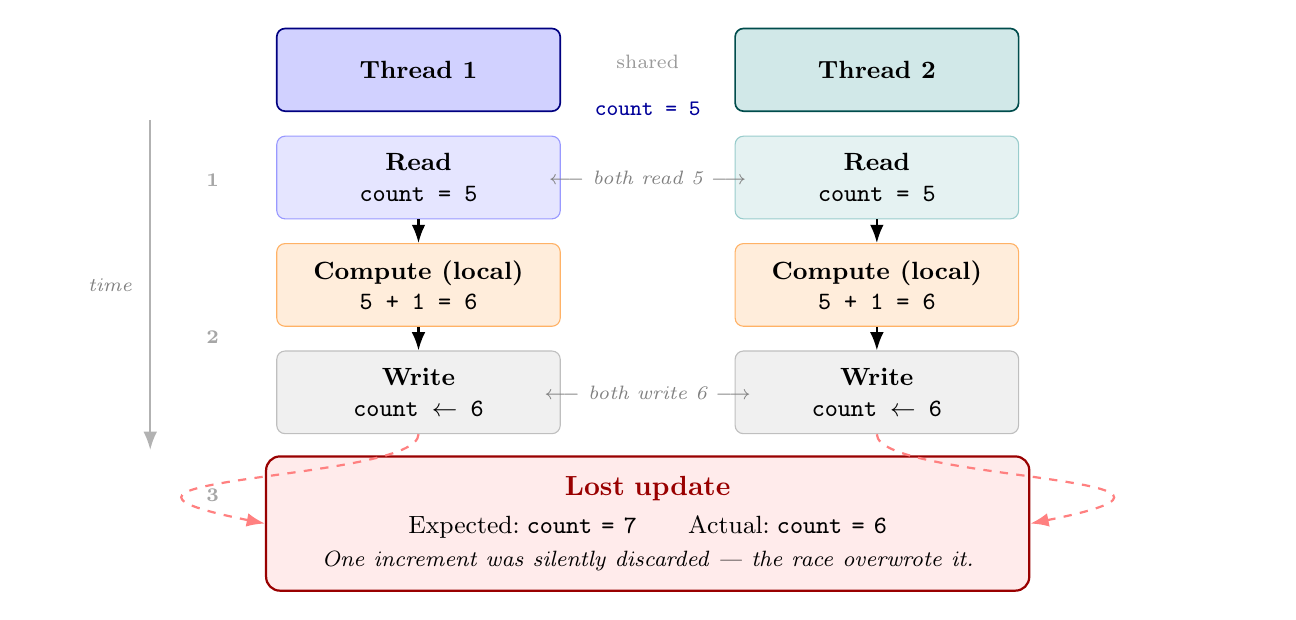
\begin{tikzpicture}[
				node distance=3mm and 22mm,
				stepbox/.style={draw, rounded corners=3pt, align=center,
					inner sep=5pt, minimum width=3.6cm, minimum height=1.05cm,
					font=\small},
				label/.style={font=\scriptsize\itshape, text=gray},
				stepnum/.style={font=\scriptsize\bfseries, text=gray!70},
				]
				
				%% ── Column headers ──────────────────────────────────────────────
				\node[stepbox, fill=blue!18, draw=blue!50!black, line width=0.6pt,
				font=\small\bfseries] (h1) {Thread 1};
				
				\node[stepbox, fill=teal!18, draw=teal!60!black, line width=0.6pt,
				font=\small\bfseries, right=of h1] (h2) {Thread 2};
				
				%% ── Step labels (left margin) ───────────────────────────────────
				\node[stepnum, left=6mm of h1, yshift=-14mm] {1};
				\node[stepnum, left=6mm of h1, yshift=-34mm] {2};
				\node[stepnum, left=6mm of h1, yshift=-54mm] {3};
				
				%% ── STEP 1: Read ────────────────────────────────────────────────
				\node[stepbox, fill=blue!10, draw=blue!40, below=3mm of h1] (t1r)
				{\textbf{Read}\\\texttt{count = 5}};
				
				\node[stepbox, fill=teal!10, draw=teal!40, below=3mm of h2] (t2r)
				{\textbf{Read}\\\texttt{count = 5}};
				
				%% ── STEP 2: Compute ─────────────────────────────────────────────
				\node[stepbox, fill=orange!14, draw=orange!60, below=of t1r] (t1c)
				{\textbf{Compute (local)}\\\texttt{5 + 1 = 6}};
				
				\node[stepbox, fill=orange!14, draw=orange!60, below=of t2r] (t2c)
				{\textbf{Compute (local)}\\\texttt{5 + 1 = 6}};
				
				%% ── STEP 3: Write ───────────────────────────────────────────────
				\node[stepbox, fill=gray!12, draw=gray!50, below=of t1c] (t1w)
				{\textbf{Write}\\\texttt{count \(\leftarrow\) 6}};
				
				\node[stepbox, fill=gray!12, draw=gray!50, below=of t2c] (t2w)
				{\textbf{Write}\\\texttt{count \(\leftarrow\) 6}};
				
				%% ── Vertical flow arrows ────────────────────────────────────────
				\draw[arrow] (t1r) -- (t1c);
				\draw[arrow] (t1c) -- (t1w);
				\draw[arrow] (t2r) -- (t2c);
				\draw[arrow] (t2c) -- (t2w);
				
				%% ── Time axis ───────────────────────────────────────────────────
				\coordinate (axistop) at ([xshift=-16mm, yshift=2mm] t1r.north west);
				\coordinate (axisbot) at ([xshift=-16mm, yshift=-2mm] t1w.south west);
				\draw[arrow, gray!60] (axistop) -- (axisbot)
				node[midway, left=1mm, font=\scriptsize\itshape, text=gray] {time};
				
				%% ── Shared-memory annotations (centre column) ───────────────────
				\coordinate (mid12) at ($(h1.east)!0.5!(h2.west)$);
				
				% "shared: count = 5" label between headers
				\node[font=\scriptsize, text=gray!80, align=center]
				at ([yshift=1mm] mid12) {shared};
				\node[font=\footnotesize\ttfamily, text=blue!60!black]
				at ([yshift=-5mm] mid12) {count = 5};
				
				% "both read 5" annotation at read level
				\node[font=\scriptsize\itshape, text=gray, align=center]
				at ($(t1r)!0.5!(t2r)$) {\(\longleftarrow\) both read 5 \(\longrightarrow\)};
				
				% "both write 6" annotation at write level
				\node[font=\scriptsize\itshape, text=gray, align=center]
				at ($(t1w)!0.5!(t2w)$) {\(\longleftarrow\) both write 6 \(\longrightarrow\)};
				
				%% ── Result box ──────────────────────────────────────────────────
				\node[draw=red!60!black, fill=red!8, rounded corners=5pt,
				text width=9.2cm, align=center,
				inner sep=7pt, line width=0.8pt,
				below=8mm of $(t1w)!0.5!(t2w)$] (result)
				{
					\textcolor{red!60!black}{\textbf{Lost update}}\\[3pt]
					\small
					Expected:\;\texttt{count = 7}\qquad
					Actual:\;\texttt{count = 6}\\
					\footnotesize\itshape
					One increment was silently discarded --- the race overwrote it.
				};
				
				\draw[dashedarrow, red!50] (t1w.south) .. controls +(0,-6mm) and +(-30mm,6mm) .. (result.west);
				\draw[dashedarrow, red!50] (t2w.south) .. controls +(0,-6mm) and +(30mm,6mm) .. (result.east);
			\end{tikzpicture}
		\end{center}
		
	\end{frame}
	
	% ============================================================
	\begin{frame}{Quick Checkpoint}
		\begin{alertblock}{Think-Pair-Share}
			If two threads withdraw \$10 from a bank account with a \$15 balance,
			and there is no synchronization, what final balances are possible?
		\end{alertblock}
		
		\bigskip
		Think about:
		\begin{itemize}
			\item What each thread may read
			\item Whether both threads may believe the withdrawal is valid
			\item Which invariant is broken
		\end{itemize}
	\end{frame}
	
	% ============================================================
	\begin{frame}{Bank Account Race --- One Unsafe Interleaving}
		
		\begin{center}
			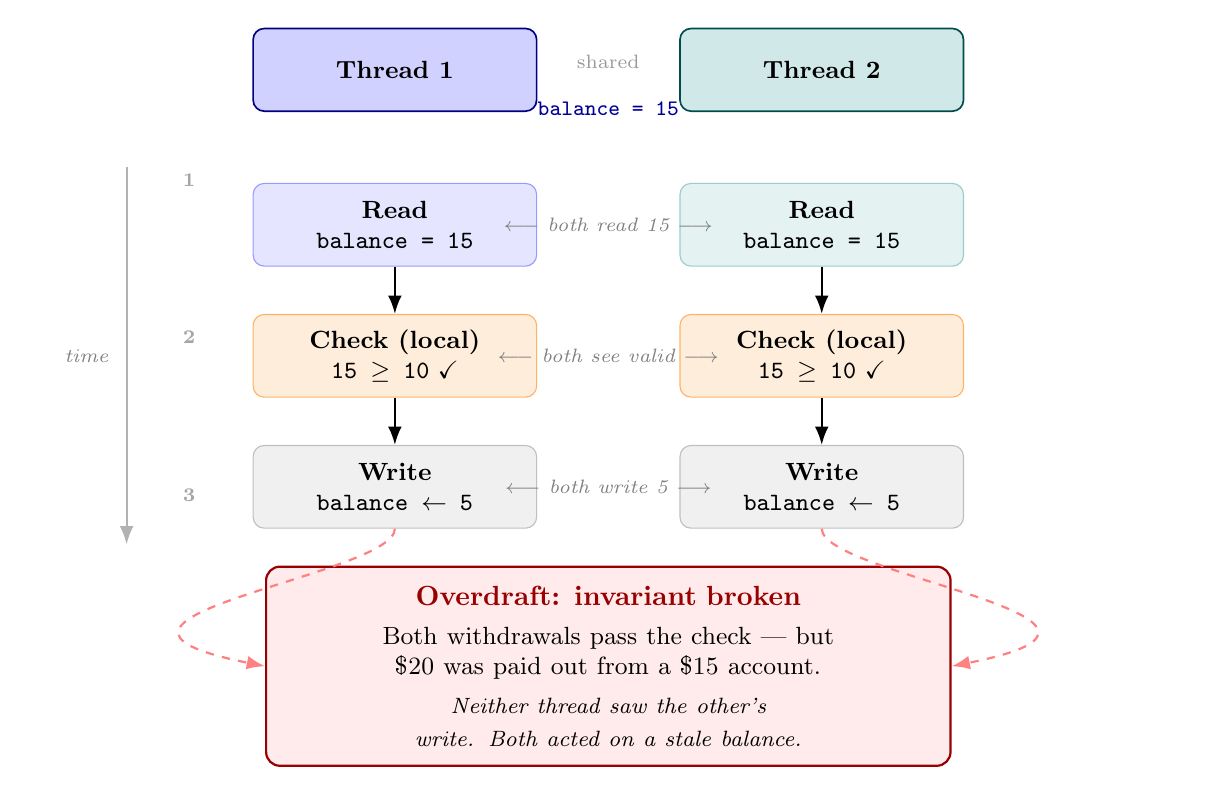
\begin{tikzpicture}[
				node distance=6mm and 18mm,
				stepbox/.style={draw, rounded corners=4pt, align=center,
					inner sep=5pt, minimum width=3.6cm, minimum height=1.05cm,
					font=\small},
				stepnum/.style={font=\scriptsize\bfseries, text=gray!70},
				]
				
				%% -- Column headers
				\node[stepbox, fill=blue!18, draw=blue!50!black, line width=0.6pt,
				font=\small\bfseries] (h1) {Thread 1};
				
				\node[stepbox, fill=teal!18, draw=teal!60!black, line width=0.6pt,
				font=\small\bfseries, right=of h1] (h2) {Thread 2};
				
				%% -- Step numbers (left margin)
				\node[stepnum, left=6mm of h1, yshift=-14mm] {1};
				\node[stepnum, left=6mm of h1, yshift=-34mm] {2};
				\node[stepnum, left=6mm of h1, yshift=-54mm] {3};
				
				%% -- STEP 1: Read
				\node[stepbox, fill=blue!10, draw=blue!40, below=9mm of h1] (t1r)
				{\textbf{Read}\\\texttt{balance = 15}};
				
				\node[stepbox, fill=teal!10, draw=teal!40, below=9mm of h2] (t2r)
				{\textbf{Read}\\\texttt{balance = 15}};
				
				%% -- STEP 2: Check
				\node[stepbox, fill=orange!14, draw=orange!60, below=of t1r] (t1c)
				{\textbf{Check (local)}\\\texttt{15 \(\ge\) 10} \checkmark};
				
				\node[stepbox, fill=orange!14, draw=orange!60, below=of t2r] (t2c)
				{\textbf{Check (local)}\\\texttt{15 \(\ge\) 10} \checkmark};
				
				%% -- STEP 3: Write
				\node[stepbox, fill=gray!12, draw=gray!50, below=of t1c] (t1w)
				{\textbf{Write}\\\texttt{balance \(\leftarrow\) 5}};
				
				\node[stepbox, fill=gray!12, draw=gray!50, below=of t2c] (t2w)
				{\textbf{Write}\\\texttt{balance \(\leftarrow\) 5}};
				
				%% -- Vertical flow arrows
				\draw[arrow] (t1r) -- (t1c);
				\draw[arrow] (t1c) -- (t1w);
				\draw[arrow] (t2r) -- (t2c);
				\draw[arrow] (t2c) -- (t2w);
				
				%% -- Time axis
				\coordinate (axistop) at ([xshift=-16mm, yshift=2mm] t1r.north west);
				\coordinate (axisbot) at ([xshift=-16mm, yshift=-2mm] t1w.south west);
				\draw[arrow, gray!60] (axistop) -- (axisbot)
				node[midway, left=1mm, font=\scriptsize\itshape, text=gray] {time};
				
				%% -- Shared-memory annotations (centre column)
				\coordinate (mid12) at ($(h1.east)!0.5!(h2.west)$);
				
				\node[font=\scriptsize, text=gray!80, align=center]
				at ([yshift=1mm] mid12) {shared};
				\node[font=\footnotesize\ttfamily, text=blue!60!black]
				at ([yshift=-5mm] mid12) {balance = 15};
				
				\node[font=\scriptsize\itshape, text=gray, align=center]
				at ($(t1r)!0.5!(t2r)$) {\(\longleftarrow\) both read 15 \(\longrightarrow\)};
				
				\node[font=\scriptsize\itshape, text=gray, align=center]
				at ($(t1c)!0.5!(t2c)$) {\(\longleftarrow\) both see valid \(\longrightarrow\)};
				
				\node[font=\scriptsize\itshape, text=gray, align=center]
				at ($(t1w)!0.5!(t2w)$) {\(\longleftarrow\) both write 5 \(\longrightarrow\)};
				
				%% -- Result box
				\node[draw=red!60!black, fill=red!8, rounded corners=5pt,
				text width=8.2cm, align=center,
				inner sep=7pt, line width=0.8pt,
				below=10mm of $(t1w)!0.5!(t2w)$] (res)
				{
					\textcolor{red!60!black}{\textbf{Overdraft: invariant broken}}\\[3pt]
					\small
					Both withdrawals pass the check --- but \$20 was paid out from a \$15 account.\\[2pt]
					\footnotesize\itshape
					Neither thread saw the other's write. Both acted on a stale balance.
				};
				
				\draw[dashedarrow, red!50] (t1w.south) .. controls +(0,-6mm) and +(-30mm,6mm) .. (res.west);
				\draw[dashedarrow, red!50] (t2w.south) .. controls +(0,-6mm) and +(30mm,6mm) .. (res.east);
				
			\end{tikzpicture}
		\end{center}
		
	\end{frame}
	
	% ============================================================
	\begin{frame}{Mental Model of the Problem}
		
		\begin{center}
			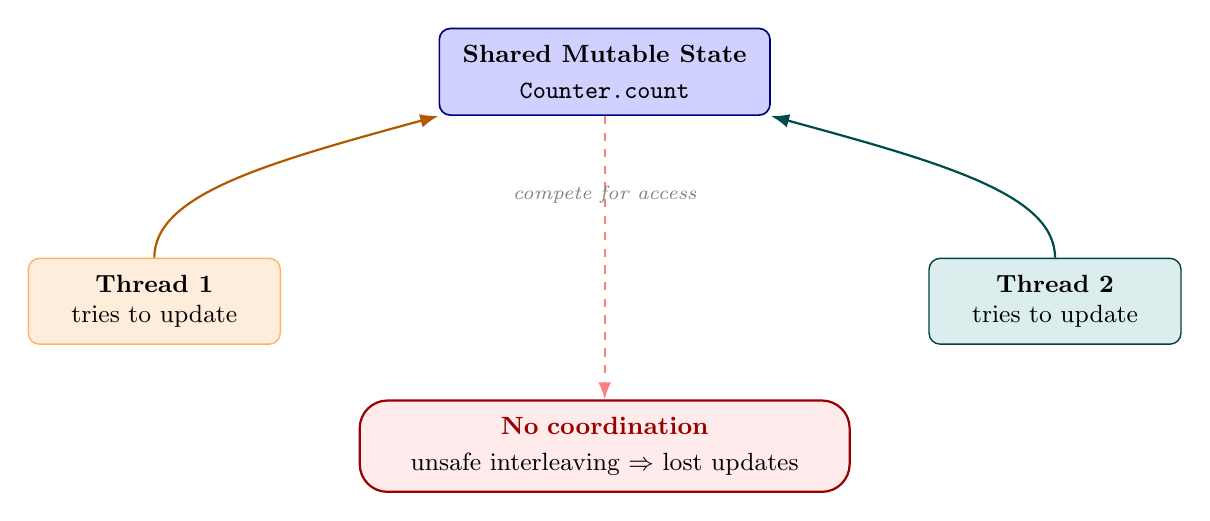
\begin{tikzpicture}[
				node distance=8mm,
				stepbox/.style={draw, rounded corners=4pt, align=center,
					inner sep=6pt, font=\small},
				pillbox/.style={draw, rounded corners=10pt, align=center,
					inner sep=6pt, font=\small},
				]
				
				%% -- Shared state (top, centre)
				\node[stepbox, fill=blue!18, draw=blue!50!black, line width=0.6pt,
				minimum width=4.2cm, minimum height=1.1cm] (shared)
				{
					\textbf{Shared Mutable State}\\[2pt]
					\texttt{\small Counter.count}
				};
				
				%% -- Thread nodes (below-left and below-right)
				\node[stepbox, fill=orange!14, draw=orange!60, line width=0.5pt,
				minimum width=3.2cm, minimum height=1.0cm,
				below left=18mm and 20mm of shared] (th1)
				{
					\textbf{Thread 1}\\
					\small tries to update
				};
				
				\node[stepbox, fill=teal!14, draw=teal!50!black, line width=0.5pt,
				minimum width=3.2cm, minimum height=1.0cm,
				below right=18mm and 20mm of shared] (th2)
				{
					\textbf{Thread 2}\\
					\small tries to update
				};
				
				%% -- Chaos pill (bottom centre, between the two threads)
				\node[pillbox, fill=red!8, draw=red!60!black, line width=0.8pt,
				text width=5.8cm, minimum height=1.0cm,
				below=36mm of shared] (chaos)
				{
					\textcolor{red!60!black}{\textbf{No coordination}}\\[2pt]
					\small unsafe interleaving \(\Rightarrow\) lost updates
				};
				
				%% -- Arrows: threads reach UP to shared state
				\draw[arrow, orange!70!black] (th1.north) .. controls +(0,8mm) and +(-22mm,-6mm) .. (shared.south west);
				\draw[arrow, teal!60!black]   (th2.north) .. controls +(0,8mm) and +(22mm,-6mm)  .. (shared.south east);
				
				%% -- Dashed arrow: shared state leads DOWN to chaos
				\draw[dashedarrow, red!50, line width=0.7pt]
				(shared.south) -- ++(0,-10mm) -- (chaos.north);
				
				%% -- Annotation: "compete for access"
				\node[font=\scriptsize\itshape, text=gray, align=center]
				at ($(th1.north east)!0.5!(th2.north west)+(0,8mm)$)
				{compete for access};
				
			\end{tikzpicture}
		\end{center}
		
		\vspace{0.2cm}
		\begin{block}{Observation}
			The problem is not randomness in Java.\\
			The problem is \textbf{unsynchronized access} to shared mutable state.
		\end{block}
		
	\end{frame}
	
	% ============================================================
	\begin{frame}{From Chaos to Control}
		\begin{block}{Problem}
			Multiple threads access the same mutable state without coordination.
		\end{block}
		
		\vspace{0.3cm}
		\begin{alertblock}{Question}
			How do we prevent this chaos?
		\end{alertblock}
		
		\vspace{0.3cm}
		\centering
		\Large We need \textbf{mutual exclusion}.
	\end{frame}
	
	% ============================================================
	\begin{frame}{A Simple Analogy for a Lock}
		\begin{block}{Analogy}
			A lock is like a room with a single key.
		\end{block}
		
		\begin{itemize}
			\item If one person holds the key, only that person may enter
			\item Everyone else must wait outside
			\item When the key is returned, another person may enter
		\end{itemize}
		
		\vspace{0.3cm}
		\begin{alertblock}{Mapping}
			Thread = person \hspace{0.5cm}
			Lock = key \hspace{0.5cm}
			Critical section = room
		\end{alertblock}
	\end{frame}
	
	% ============================================================
	\begin{frame}[fragile]{Introducing \texttt{synchronized}}
		\begin{lstlisting}[language=Java]
			synchronized(lockObject) {
				// critical section
			}
		\end{lstlisting}
		
		\bigskip
		\begin{block}{Behavioral Guarantee}
			Only one thread executes inside the critical section at a time,
			provided all threads synchronize on the same lock object.
		\end{block}
		
		\bigskip
		This is \textbf{mutual exclusion}.
	\end{frame}
	
	% ============================================================
	\begin{frame}[fragile]{\texttt{synchronized} Method vs Block}
		\begin{lstlisting}[language=Java]
			public synchronized void increment() {
				count++;
			}
		\end{lstlisting}
		
		\vspace{0.2cm}
		
		\begin{lstlisting}[language=Java]
			public void increment() {
				synchronized(this) {
					count++;
				}
			}
		\end{lstlisting}
		
		\vspace{0.3cm}
		\begin{block}{Key idea}
			For an instance method, \texttt{synchronized} uses the monitor of \texttt{this}.
		\end{block}
		
		\begin{alertblock}{Important}
			A synchronized block gives more control because you choose the lock object explicitly.
		\end{alertblock}
	\end{frame}
	
	% ============================================================
	\begin{frame}{What Is a Monitor?}
		\begin{block}{Main Idea}
			In Java, every object has an intrinsic monitor.
		\end{block}
		
		\begin{itemize}
			\item A thread can acquire the monitor
			\item Other threads trying to enter become blocked
			\item The monitor is released when the synchronized region exits
		\end{itemize}
		
		\bigskip
		\begin{alertblock}{Key Point}
			Synchronization works through object identity.
		\end{alertblock}
	\end{frame}
	
	% ============================================================
	\begin{frame}{Concept Check --- BLOCKED vs WAITING}
		\begin{block}{BLOCKED}
			A thread is \textbf{BLOCKED} when it is trying to enter a
			\texttt{synchronized} region but another thread already holds the monitor.
		\end{block}
		
		\vspace{0.3cm}
		\begin{block}{WAITING}
			A thread is \textbf{WAITING} when it has voluntarily paused,
			typically as part of condition coordination such as \texttt{wait()}.
		\end{block}
		
		\vspace{0.3cm}
		\begin{alertblock}{For today}
			We focus on monitor contention and BLOCKED threads.
			Condition waiting will be treated later.
		\end{alertblock}
	\end{frame}
	% ============================================================
	\begin{frame}{Monitor Layout (Conceptual View)}
		
		\begin{center}
			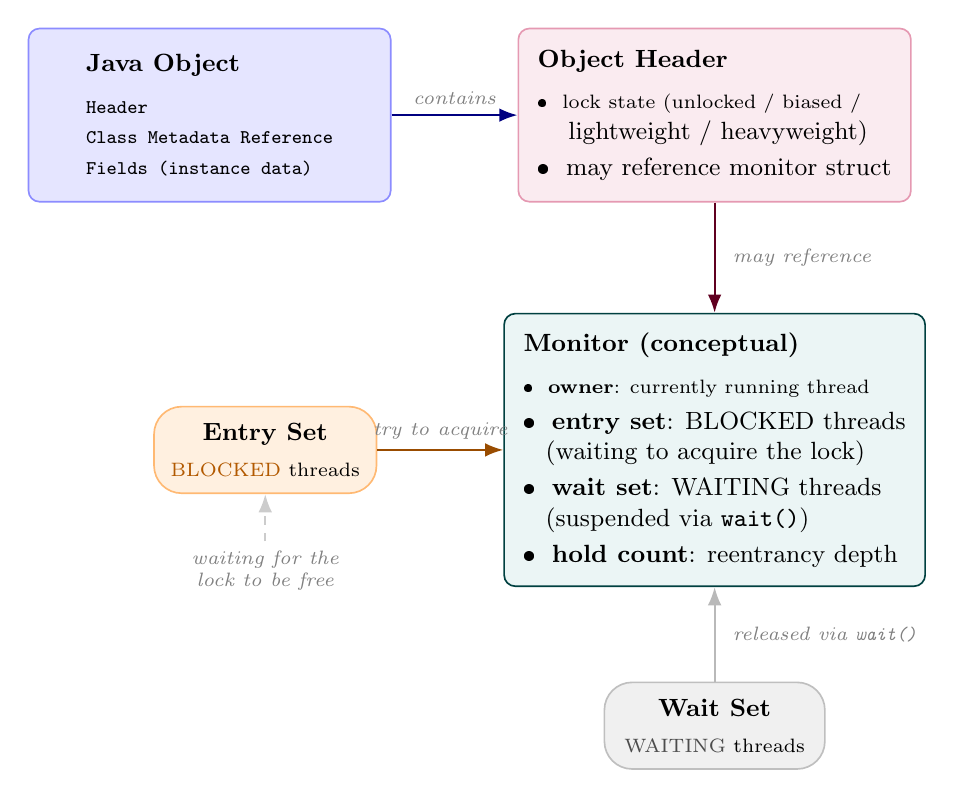
\begin{tikzpicture}[
				node distance=7mm and 14mm,
				stepbox/.style={draw, rounded corners=4pt, align=left,
					inner sep=7pt, font=\small},
				pillbox/.style={draw, rounded corners=10pt, align=center,
					inner sep=6pt, font=\small},
				tinylabel/.style={font=\scriptsize\itshape, text=gray},
				]
				
				%% ── Java Object (top-left) ───────────────────────────────────────
				\node[stepbox, fill=blue!10, draw=blue!45, line width=0.6pt,
				minimum width=4.6cm, minimum height=2.2cm] (obj)
				{
					\textbf{Java Object}\\[4pt]
					\texttt{\scriptsize Header}\\
					\texttt{\scriptsize Class Metadata Reference}\\
					\texttt{\scriptsize Fields (instance data)}
				};
				
				%% ── Header / Lock Word (top-right) ──────────────────────────────
				\node[stepbox, fill=purple!8, draw=purple!40, line width=0.6pt,
				minimum width=4.6cm, minimum height=2.2cm,
				right=16mm of obj] (mark)
				{
					\textbf{Object Header}\\[4pt]
					\scriptsize
					\textbullet\; lock state (unlocked / biased /\\
					\hspace{8pt} lightweight / heavyweight)\\[2pt]
					\textbullet\; may reference monitor struct
				};
				
				\draw[arrow, blue!50!black] (obj.east) --
				node[above, tinylabel]{contains} (mark.west);
				
				%% ── Monitor box (bottom-right, below header) ─────────────────────
				\node[stepbox, fill=teal!8, draw=teal!50!black, line width=0.6pt,
				minimum width=4.6cm, minimum height=3.0cm,
				below=14mm of mark] (mon)
				{
					\textbf{Monitor (conceptual)}\\[4pt]
					\scriptsize
					\textbullet\; \textbf{owner}: currently running thread\\[2pt]
					\textbullet\; \textbf{entry set}: BLOCKED threads\\
					\hspace{8pt}(waiting to acquire the lock)\\[2pt]
					\textbullet\; \textbf{wait set}: WAITING threads\\
					\hspace{8pt}(suspended via \texttt{wait()})\\[2pt]
					\textbullet\; \textbf{hold count}: reentrancy depth
				};
				
				\draw[arrow, purple!50!black] (mark.south) --
				node[right=1mm, tinylabel]{may reference} (mon.north);
				
				%% ── Entry Set pill (left of monitor) ────────────────────────────
				\node[pillbox, fill=orange!12, draw=orange!55, line width=0.6pt,
				minimum width=2.8cm, minimum height=1.1cm,
				left=16mm of mon] (entry)
				{
					\textbf{Entry Set}\\[2pt]
					\scriptsize\textcolor{orange!70!black}{BLOCKED} threads
				};
				
				%% ── Wait Set pill (below monitor) ───────────────────────────────
				\node[pillbox, fill=gray!12, draw=gray!50, line width=0.6pt,
				minimum width=2.8cm, minimum height=1.1cm,
				below=12mm of mon] (waits)
				{
					\textbf{Wait Set}\\[2pt]
					\scriptsize\textcolor{gray!60!black}{WAITING} threads
				};
				
				%% ── Arrows: sets connect to monitor ─────────────────────────────
				\draw[arrow, orange!60!black] (entry.east) --
				node[above, tinylabel]{try to acquire} (mon.west);
				
				\draw[arrow, gray!55] (waits.north) --
				node[right=1mm, tinylabel]{released via \texttt{wait()}} (mon.south);
				
				%% ── Annotation: BLOCKED vs WAITING distinction ───────────────────
				\node[font=\scriptsize\itshape, text=gray, align=center,
				below=6mm of entry] (note)
				{
					waiting for the\\lock to be free
				};
				\draw[dashedarrow, gray!40] (note.north) -- (entry.south);
				
			\end{tikzpicture}
		\end{center}
		
	\end{frame}
	% ============================================================
	\begin{frame}{Reentrancy in One Sentence}
		\begin{block}{Reentrancy}
			If a thread already holds a monitor, it may enter another
			\texttt{synchronized} region guarded by the same object
			without blocking itself.
		\end{block}
		
		\vspace{0.3cm}
		\begin{alertblock}{Why it matters}
			Without reentrancy, many ordinary object-oriented method calls
			would deadlock immediately.
		\end{alertblock}
	\end{frame}
	
	\begin{frame}{Visibility Intuition --- Caches and Main Memory}
		\centering
		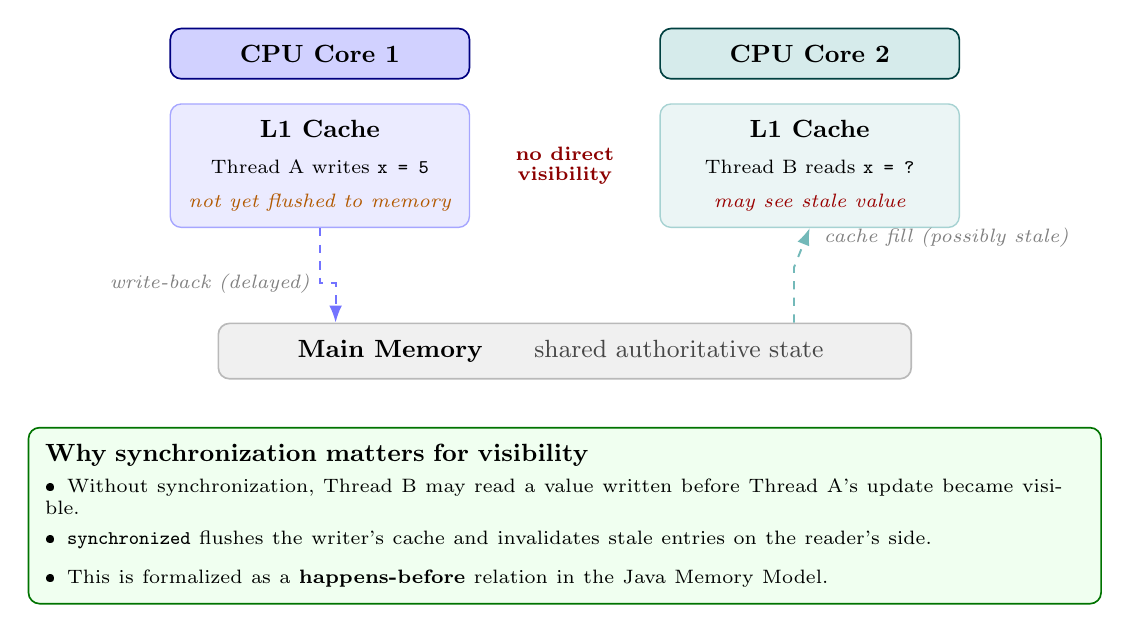
\begin{tikzpicture}[
			stepbox/.style={
				draw, rounded corners=4pt, align=center,
				inner sep=6pt, font=\small
			}
			]
			
			%% -- CPU Core 1 (left)
			\node[stepbox, fill=blue!18, draw=blue!50!black, line width=0.6pt,
			minimum width=3.8cm] (core1)
			{\textbf{CPU Core 1}};
			
			\node[stepbox, fill=blue!8, draw=blue!35, line width=0.5pt,
			minimum width=3.8cm, below=3mm of core1] (cache1)
			{
				\textbf{L1 Cache}\\[2pt]
				\scriptsize Thread A writes \texttt{x = 5}\\[1pt]
				\scriptsize\textcolor{orange!70!black}{\itshape not yet flushed to memory}
			};
			
			%% -- CPU Core 2 (right)
			\node[stepbox, fill=teal!16, draw=teal!50!black, line width=0.6pt,
			minimum width=3.8cm, right=24mm of core1] (core2)
			{\textbf{CPU Core 2}};
			
			\node[stepbox, fill=teal!8, draw=teal!35, line width=0.5pt,
			minimum width=3.8cm, below=3mm of core2] (cache2)
			{
				\textbf{L1 Cache}\\[2pt]
				\scriptsize Thread B reads \texttt{x = ?}\\[1pt]
				\scriptsize\textcolor{red!60!black}{\itshape may see stale value}
			};
			
			%% -- "no direct visibility" badge
			\node[font=\scriptsize\bfseries, text=red!55!black, align=center]
			at ($(cache1.east)!0.5!(cache2.west)$)
			{no direct\\[-1pt]visibility};
			
			%% -- Main Memory
			\path (cache1.south) -- (cache2.south) coordinate[midway] (mid);
			\node[stepbox, fill=gray!12, draw=gray!55, line width=0.6pt,
			minimum width=8.8cm, below=12mm of mid] (ram)
			{
				\textbf{Main Memory}\qquad
				\textcolor{gray!55!black}{\small shared authoritative state}
			};
			
			%% -- Write path: cache1 down to RAM (left side)
			\draw[dashed, -Latex, blue!55, line width=0.7pt]
			(cache1.south) -- ++(0,-7mm) -| ([xshift=15mm]ram.north west)
			node[pos=0.25, left=1mm, font=\scriptsize\itshape, text=gray]
			{write-back (delayed)};
			
			%% -- Read path: RAM (right side) up to cache2
			\draw[dashed, -Latex, teal!55, line width=0.7pt]
			([xshift=-15mm]ram.north east) |- ++(0,7mm) -- (cache2.south)
			node[pos=0.75, right=1mm, font=\scriptsize\itshape, text=gray]
			{cache fill (possibly stale)};
			
			%% -- Takeaway box
			\node[stepbox, fill=green!6, draw=green!45!black, line width=0.6pt,
			text width=13.2cm, align=left, below=6mm of ram]
			{
				\textbf{Why synchronization matters for visibility}\\[3pt]
				\scriptsize
				\textbullet\enspace Without synchronization, Thread B may read a value
				written before Thread A's update became visible.\\[3pt]
				\textbullet\enspace \texttt{synchronized} flushes the writer's cache and
				invalidates stale entries on the reader's side.\\[3pt]
				\textbullet\enspace This is formalized as a \textbf{happens-before}
				relation in the Java Memory Model.
			};
			
		\end{tikzpicture}
	\end{frame}
	% ============================================================
	\begin{frame}{Connecting Back to the Race}
		The counter failed because:
		\begin{itemize}
			\item operations interleaved without mutual exclusion
			\item no synchronization guaranteed visibility between threads
		\end{itemize}
		
		\bigskip
		\begin{block}{Important}
			Monitors are not only about blocking overlap.
			They also support memory visibility guarantees in the Java Memory Model.
		\end{block}
		
		\bigskip
		\begin{alertblock}{Bridge to next part}
			In the Java Memory Model, synchronization establishes
			a \textbf{happens-before} relationship between threads.
		\end{alertblock}
	\end{frame}
	
	% ============================================================
	\begin{frame}[fragile]{Protecting the Counter with a Shared Lock}
		\begin{lstlisting}[language=Java]
			class Counter {
				static int count = 0;
				static final Object lock = new Object();
				
				static void increment() {
					synchronized(lock) {
						count++;
					}
				}
			}
		\end{lstlisting}
		
		\vspace{0.2cm}
		\begin{block}{Interpretation}
			The increment is now protected by one shared monitor.
			Only one thread may execute that critical section at a time.
		\end{block}
	\end{frame}
	
	% ============================================================
	\begin{frame}[fragile]{Lock Identity Trap}
		\begin{lstlisting}[language=Java]
			public void withdraw(int amount) {
				Object lock = new Object();
				synchronized(lock) {
					balance -= amount;
				}
			}
		\end{lstlisting}
		
		\bigskip
		\begin{alertblock}{Question}
			Why does this fail to protect \texttt{balance}?
		\end{alertblock}
	\end{frame}
	
	% ============================================================
	\begin{frame}{The Lock Identity Rule}
		Each call creates a new lock object.
		
		\bigskip
		Different threads therefore lock different objects.
		
		\bigskip
		\begin{alertblock}{Critical Rule}
			Synchronization works only when all threads lock the \textbf{same identity}.
		\end{alertblock}
	\end{frame}
	
	% ============================================================
	\begin{frame}[fragile]{Spot the Bug}
		\begin{lstlisting}[language=Java]
			class Counter {
				private int count = 0;
				
				public void increment() {
					synchronized(new Object()) {
						count++;
					}
				}
			}
		\end{lstlisting}
		
		\vspace{0.2cm}
		\begin{block}{Answer}
			This creates a fresh lock object every time.
			No shared monitor means no real coordination.
		\end{block}
	\end{frame}
	
	% ============================================================
	\begin{frame}{A Common Misconception}
		\begin{alertblock}{Important}
			Synchronizing one method does not automatically make
			all related code thread-safe.
		\end{alertblock}
		
		\vspace{0.3cm}
		\begin{itemize}
			\item All access paths to shared mutable state matter
			\item Reads may also require synchronization
			\item Thread safety is a property of the design, not one keyword
		\end{itemize}
	\end{frame}
	
	% ============================================================
	\begin{frame}{Reflection}
		How does the distinction between:
		\begin{itemize}
			\item BLOCKED
			\item WAITING
		\end{itemize}
		relate to:
		\begin{itemize}
			\item protecting a shared monitor identity
			\item waiting for a condition via \texttt{wait()} / \texttt{notify()}
		\end{itemize}
		
		\bigskip
		Write one sentence connecting the concepts.
	\end{frame}
	
	% ============================================================
	\begin{frame}{Takeaways}
		\begin{itemize}
			\item Race conditions come from unsynchronized access to shared mutable state
			\item \texttt{count++} is not atomic
			\item \texttt{synchronized} provides mutual exclusion
			\item Every Java object has an intrinsic monitor
			\item Synchronization depends on \textbf{shared lock identity}
			\item Synchronization also supports visibility guarantees
		\end{itemize}
		
		\vspace{0.3cm}
		\begin{alertblock}{Next}
			We now go deeper into what \texttt{synchronized} guarantees:
			happens-before, visibility, and memory semantics.
		\end{alertblock}
	\end{frame}
	
\end{document}